% -*- latex -*-
%%%%%%%%%%%%%%%%%%%%%%%%%%%%%%%%%%%%%%%%%%%%%%%%%%%%%%%%%%%%%%%%
%%%%
%%%% This TeX file is part of the tutorial
%%%% `Introduction to the PETSc library'
%%%% Victor Eijkhout, eijkhout@tacc.utexas.edu
%%%% copyright Victor Eijkhout 2012-6
%%%%
%%%%%%%%%%%%%%%%%%%%%%%%%%%%%%%%%%%%%%%%%%%%%%%%%%%%%%%%%%%%%%%%

\sectionframe{An example program}

\begin{details}
\frame{\frametitle{Note}
This example is simplified, it is intended to convey the `taste' of
PETSc, not all the details.

However, there will be several complete examples in the lab exercises.

Also the PETSc source tree comes with many examples.
}
\end{details}

\frame[containsverbatim]{\frametitle{Create matrix}
Create distributed matrix on communicator, set local and global size.
\begin{verbatim}
  comm = MPI_COMM_WORLD; // or subset
  MatCreate(comm,&A);
  MatSetType(A,MATMPIAIJ);
  MatSetSizes(A,PETSC_DECIDE,PETSC_DECIDE,
    matrix_size,matrix_size);

  comm = MPI_COMM_WORLD ! or subset
  call MatCreate(comm,A,e) 
  call MatSetType(A,MATMPIAIJ,e)
  call MatSetSizes(A,PETSC_DECIDE,PETSC_DECIDE,
 >     matrix_size,matrix_size,e)
\end{verbatim}
}

\begin{details}
\frame{\frametitle{Parallel layout of matrices and vectors}
  \begin{itemize}
  \item local size and global size
  \item local rows contiguous
  \item matrix/vector local sizes must fit
  \item any processor can \emph{set} any matrix element
  \item processors can only \emph{inspect} local elements
  \end{itemize}
}
\end{details}

\frame{\frametitle{Parallel layout of matrices and vectors}
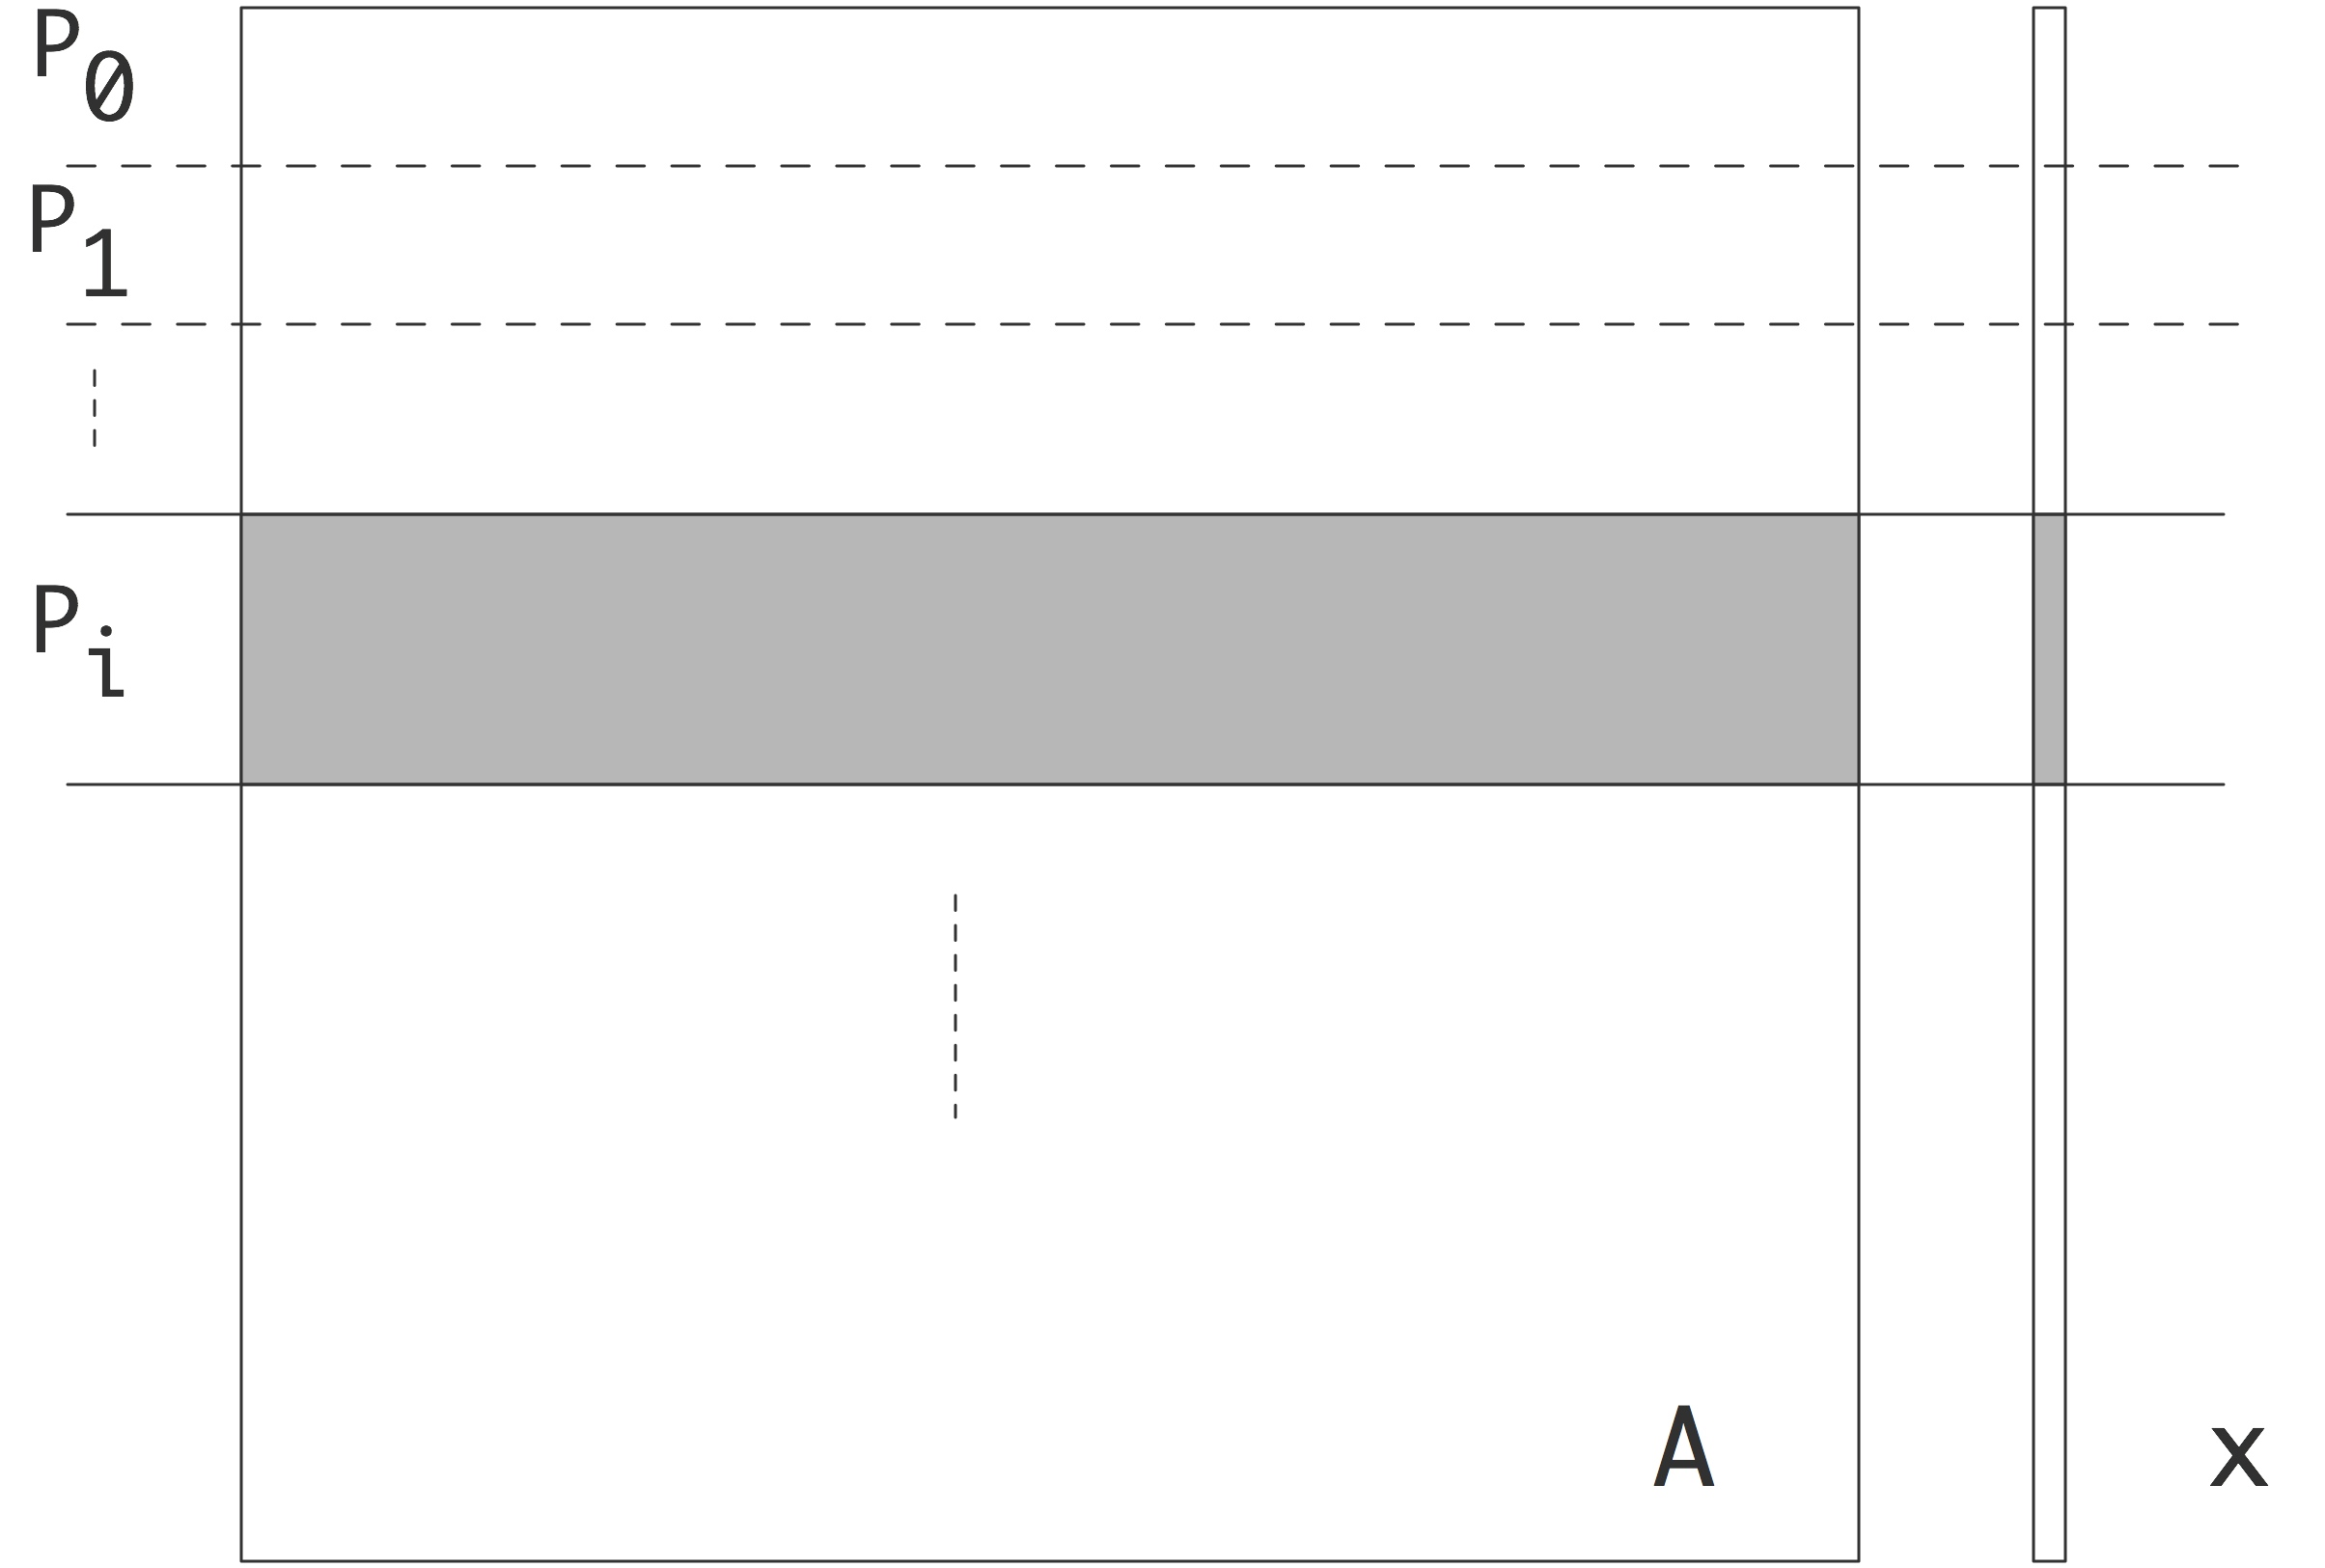
\includegraphics[scale=.1]{parallel-matrix}
}

\frame[containsverbatim]{\frametitle{Five-point Laplacian}
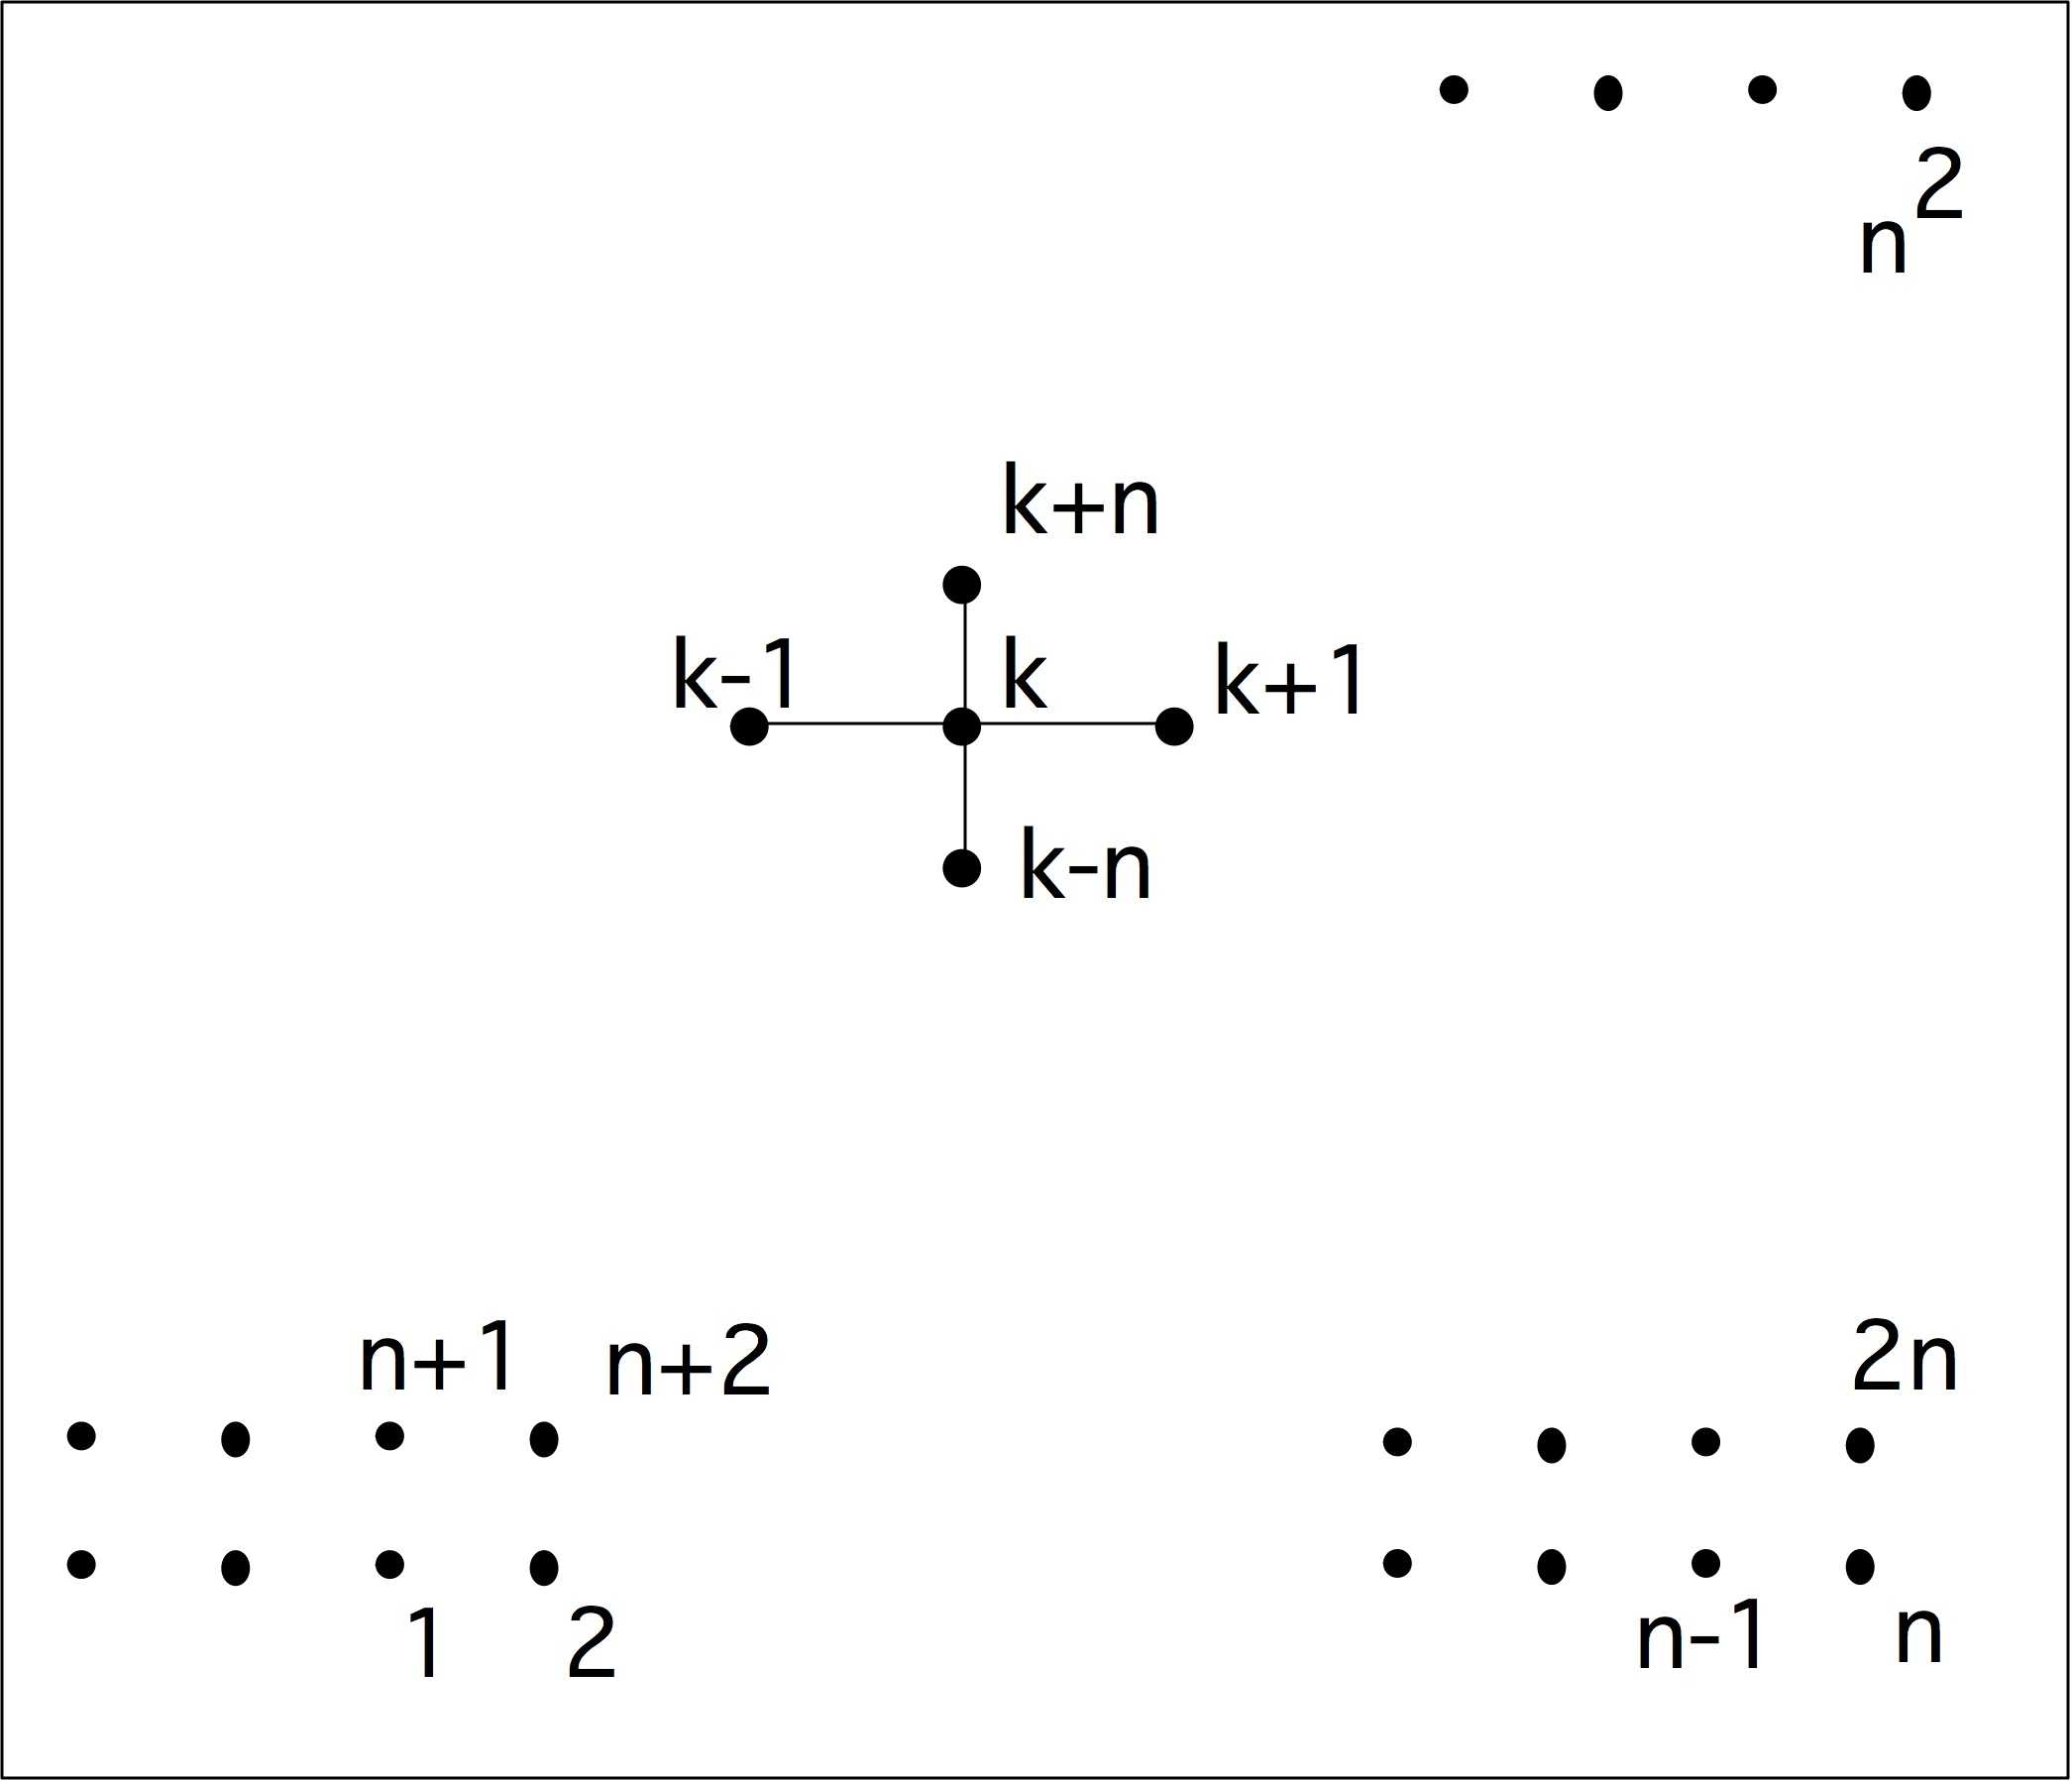
\includegraphics[scale=.06]{laplacedomain}
\hfil\break\hbox{}\hfill
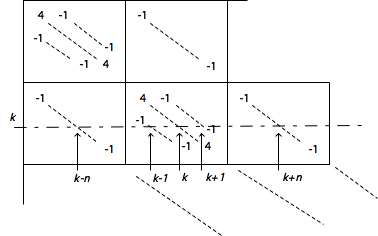
\includegraphics[scale=.6]{laplacematrix}
}

\frame[containsverbatim]{\frametitle{Fill in matrix elements (C)}
\begin{verbatim}
  MatGetOwnershipRange(A,&low,&high);
  for ( i=0; i<m; i++ ) {
    for ( j=0; j<n; j++ ) {
      Iglob = j + n*i;
      if (Iglob>=low && Iglob<high) { // my row!
        Jglob = Iglob-1; v = -1.0;
        if (i>0) MatSetValues
            (A,1,&Iglob,1,&Jglob,&v,INSERT_VALUES);
        Jglob = Iglob+1 // et cetera
      }
    }
  }
  MatAssemblyBegin(A,MAT_FINAL_ASSEMBLY);
  MatAssemblyEnd(A,MAT_FINAL_ASSEMBLY);
\end{verbatim}
Use \n{MAT_FLUSH_ASSEMBLY} if later additions
}

\frame[containsverbatim]{\frametitle{Fill in matrix elements (F)}
\begin{verbatim}
  call MatGetOwnershipRange(A,low,high,e)
  do i=0,m-1
     do j=0,n-1
        iglob = j + n*i
        if (iglob>=low .and. iglob<high) then ! my row!
           jglob = iglob - n
           if (j>0) call MatSetValues
 >             (A,1,iglob,1,jglob,v,INSERT_VALUES,e)
           ...
  call MatAssemblyBegin(A,MAT_FINAL_ASSEMBLY,e)
  call MatAssemblyEnd(A,MAT_FINAL_ASSEMBLY,e)
\end{verbatim}
}

\frame[containsverbatim]{\frametitle{Finite Element Matrix assembly}
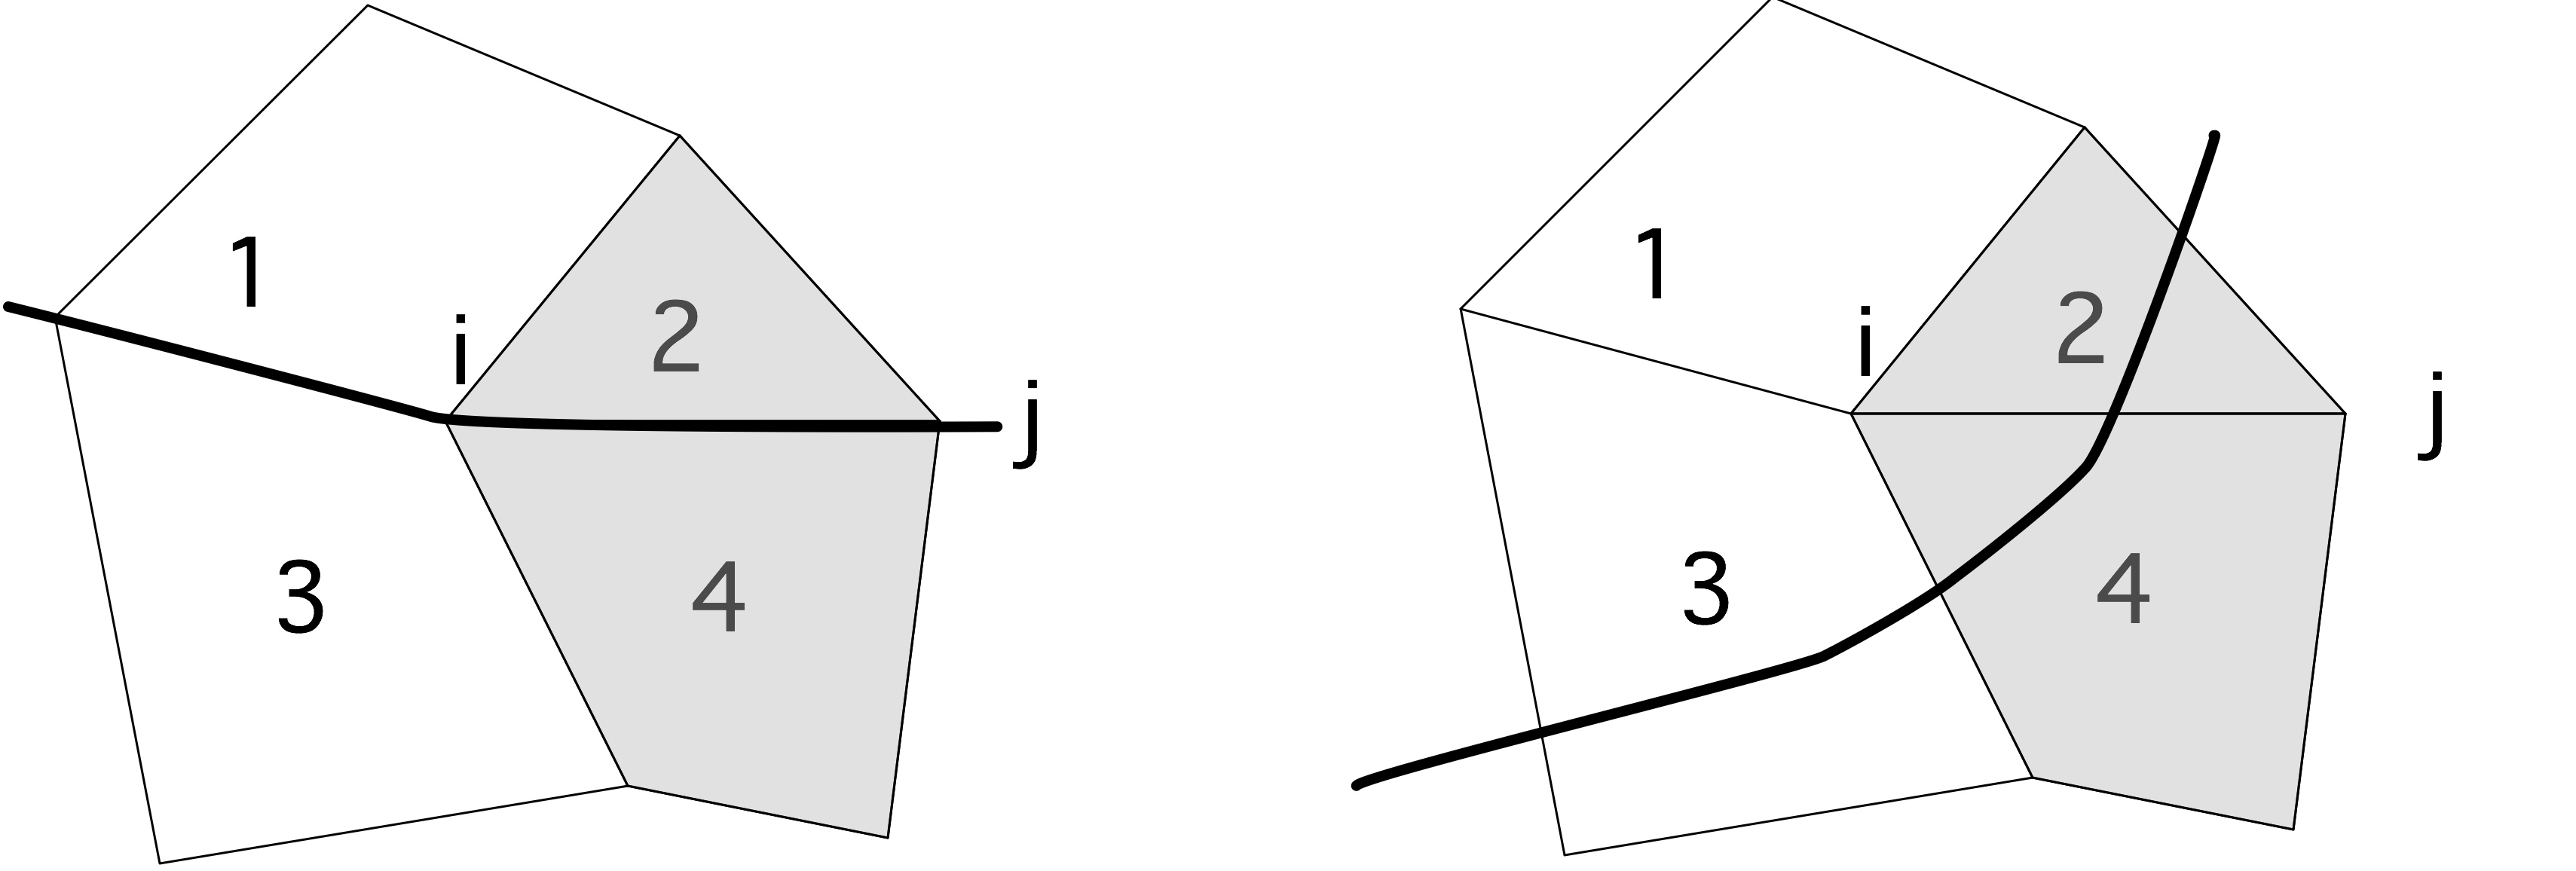
\includegraphics[scale=.1]{fem-twice}
}

\frame[containsverbatim]{\frametitle{Finite Element Matrix assembly}
\begin{verbatim}
  for (e=myfirstelement; e<mylastelement; e++) {
    for (i=0; i<nlocalnodes; i++) {
      I = localtoglobal(e,i);
      for (j=0; j<nlocalnodes; j++) {
        J = localtoglobal(e,j);
        v = integration(e,i,j);
        MatSetValues
            (mat,1,&I,1,&J,&v,ADD_VALUES);
        ....
      }
    }
  }
  MatAssemblyBegin(mat,MAT_FINAL_ASSEMBLY);
  MatAssemblyEnd(mat,MAT_FINAL_ASSEMBLY);
\end{verbatim}
}

\frame[containsverbatim]{\frametitle{Linear system solving}
System \[ Ax=b \]
Iterative methods: sequence \[ x^{0},x^{1},\ldots\longrightarrow x \]
Process depends on properties of~$A$, hence:\\
Preconditioning: \[ M\inv Ax=M\inv b \]
To be determined: 1/~iterative scheme, 2/~preconditioner
}

\frame[containsverbatim]{\frametitle{Create solver}
\begin{verbatim}
  KSPCreate(comm,&Solver);
  KSPSetOperators(Solver,A,A);
  KSPSetType(Solver,KSPCGS);
\end{verbatim}

\begin{verbatim}
  call KSPCreate(comm,Solve,e)
  call KSPSetOperators(Solve,A,A,e)
  call KSPSetType(Solve,KSPCGS,e)
\end{verbatim}
}

\frame[containsverbatim]{\frametitle{Create preconditioner}
\begin{verbatim}
  {
    PC Prec;
    KSPGetPC(Solver,&Prec);
    PCSetType(Prec,PCJACOBI);
  }
\end{verbatim}
\begin{verbatim}
  call KSPGetPC(Solve,Prec,e)
  call PCSetType(Prec,PCJACOBI,e)
\end{verbatim}
}

\frame[containsverbatim]{\frametitle{Input and output vectors}
\begin{verbatim}
  VecCreateMPI(comm,PETSC_DECIDE,matrix_size,&Rhs);
  VecDuplicate(Rhs,&Sol);
  VecSet(Rhs,one);

  call VecCreateMPI(comm,PETSC_DECIDE,matrix_size,Rhs,e)
  call VecDuplicate(Rhs,Sol,e)
  call VecSet(Rhs,one,e)
\end{verbatim}

Another way to determine the vector size:
\begin{verbatim}
  MatGetLocalSize(A,&isize,&jsize);
  VecCreateMPI(comm,isize,PETSC_DECIDE,&Rhs);
\end{verbatim}
(use \n{PETSC_NULL} instead of \n{jsize} if not interested)
}

\frame[containsverbatim]{\frametitle{Solve! (C)}
\begin{verbatim}
  KSPSolve(Solver,Rhs,Sol)
  {
    PetscInt its; KSPConvergedReason reason; 
    Vec Res; PetscReal norm;
    KSPGetConvergedReason(Solver,&reason);
    if (reason<0) {
      PetscPrintf(comm,
        "Failure to converge after %d iterations; reason %s\n",
       its,KSPConvergedReasons[reason]);
    } else {
      KSPGetIterationNumber(Solver,&its);
      PetscPrintf(comm,"Number of iterations: %d\n",its);
    }
  }
\end{verbatim}
}

\frame[containsverbatim]{\frametitle{Solve! (F)}
\begin{verbatim}
  call KSPSolve(Solve,Rhs,Sol,e)
  
  call KSPGetConvergedReason(Solve,reason,e)
  if (reason<0) then
     call PetscPrintf(comm,"Failure to converge\n",e)
  else
     call KSPGetIterationNumber(Solve,its,e)
     write(msg,10) its
10   format('Number of iterations: i4")
     call PetscPrintf(comm,msg,e)
  end if
\end{verbatim}
}

\frame[containsverbatim]{\frametitle{Quick experimentation}
Set iterative solver and preconditioner from the commandline:
\begin{verbatim}
yourprog -ksp_type gmres -ksp_gmres_restart 25
    -pc_type ilu -pc_factor_levels 3
\end{verbatim}
requires in your code:
\begin{verbatim}
KSPSetFromOptions(solver);
\end{verbatim}
}

\frame[containsverbatim]{\frametitle{Residual calculation}
\begin{verbatim}
  VecDuplicate(Rhs,&Res);
  MatMult(A,Sol,Res);
  VecAXPY(Res,-1,Rhs);
  VecNorm(Res,NORM_2,&norm);
  PetscPrintf(MPI_COMM_WORLD,"residual norm: %e\n",norm);

  call VecDuplicate(Rhs,Res,e)
  call MatMult(A,Sol,Res,e)
  call VecAXPY(Res,mone,Rhs,e)
  call VecNorm(Res,NORM_2,norm,e)
  if (mytid==0) print *,"residual norm:",norm
\end{verbatim}
}

\frame[containsverbatim]{\frametitle{Clean up}
Free all objects, both the obvious ones (matrix) and the non-obvious
ones (solver)
\begin{verbatim}
  VecDestroy(&Res);
  KSPDestroy(&Solver);
  VecDestroy(&Rhs);
  VecDestroy(&Sol);

  call MatDestroy(A,e)
  call KSPDestroy(Solve,e)
  call VecDestroy(Rhs,e)
  call VecDestroy(Sol,e)
  call VecDestroy(Res,e)
\end{verbatim}
}

